\documentclass[11pt]{article}
\usepackage[margin=1in]{geometry}
\usepackage{amsmath,amssymb,amsthm,mathtools,bm}
\usepackage{booktabs,array,tabularx}
\usepackage{tikz}
\usetikzlibrary{arrows.meta,decorations.markings,calc}
\usepackage[dvipsnames]{xcolor}
\usepackage{tcolorbox}
\usepackage[numbers,sort&compress]{natbib}
\usepackage[colorlinks=true,linkcolor=RoyalBlue,citecolor=ForestGreen,urlcolor=RoyalBlue]{hyperref}
\usepackage[capitalise]{cleveref}

% ---------- macros ----------
\newcommand{\Tr}{\operatorname{Tr}}
\newcommand{\Lc}{\mathcal{L}}
\newcommand{\Pc}{\mathcal{P}}
\newcommand{\Qc}{\mathcal{Q}}
\newcommand{\Kc}{\mathcal{K}}
\newcommand{\Gc}{\mathcal{G}}
\newcommand{\ee}{\mathrm{e}}
\newcommand{\dd}{\mathrm{d}}
\newcommand{\cl}{\mathrm{c}}
\newcommand{\qu}{\mathrm{q}}
\newcommand{\rhoS}{\rho_{S}}
\newcommand{\rhoB}{\rho_{B}}
\newcommand{\ket}[1]{|#1\rangle}
\newcommand{\bra}[1]{\langle#1|}
\newcommand{\avg}[1]{\langle#1\rangle}
\newcommand{\acomm}[2]{\{#1,#2\}}
\newcommand{\comm}[2]{[#1,#2]}

\newtcolorbox{keybox}[1][]{colback=RoyalBlue!4,colframe=RoyalBlue!60,
  fonttitle=\bfseries,title=#1,boxrule=0.6pt,arc=2pt,left=4pt,right=4pt,top=3pt,bottom=3pt}
\newtcolorbox{warnbox}{colback=Orange!6,colframe=Orange!70,boxrule=0.6pt,arc=2pt,
  left=4pt,right=4pt,top=3pt,bottom=3pt}

\newtheorem{exercise}{Exercise}

\title{\textbf{Keldysh and Mori--Zwanzig}\\[2pt]
\large Two languages for the same open-system dynamics:\\ a working note and a self-study plan}
\author{Notes prepared with Claude}
\date{30 September 2026}

\begin{document}
\maketitle

\begin{warnbox}
\small\textbf{About the references.} All bibliography entries were checked on
30~September~2026 against publisher, Crossref, or arXiv records, and DOIs were added
where they exist. The equations in the main text were derived and cross-checked
independently of the references.
\end{warnbox}

\begin{keybox}[The thesis in three lines]
\begin{enumerate}\itemsep0pt
\item \emph{Density-matrix level.} Ordering Liouville-space superoperators along a
  single real time axis \emph{is} Keldysh contour ordering. With the Nakajima projector
  $\Pc=\rhoB\otimes\Tr_B$ and a Gaussian bath, the NZ memory kernel is the
  \emph{irreducible self-energy} of the reduced propagator, and the NZ equation is a
  Dyson equation.
\item \emph{Operator level.} Mori's projection onto a system operator $A$ yields a
  generalized Langevin equation. For $A=c$ with the anticommutator inner product, the
  Mori memory function is (up to a factor $-i$) the \emph{retarded} self-energy
  $\Sigma^R$.
\item \emph{Common ground.} Both expansions are built from the two bath kernels that
  appear in the Keldysh/Feynman--Vernon influence functional: the response
  $\chi$ (retarded, $\mathrm{c}\text{--}\mathrm{q}$) and the noise $S$ (Keldysh,
  $\mathrm{c}\text{--}\mathrm{c}$). Differences between the methods come from
  \emph{which object is projected} and \emph{how the series is resummed}, not from
  different physics.
\end{enumerate}
\end{keybox}

\tableofcontents

%=====================================================================
\section{Setup and conventions}
\label{sec:setup}

We set $\hbar=1$ throughout and take
\begin{equation}
  H = H_S + H_B + H_I,\qquad H_I=\sum_\alpha S_\alpha\otimes B_\alpha ,
\end{equation}
with Hermitian $S_\alpha$, $B_\alpha$, a stationary bath state $\rhoB$ ($[H_B,\rhoB]=0$),
and $\avg{B_\alpha}\equiv\Tr_B(B_\alpha\rhoB)=0$. The Liouvillian is
$\Lc X=-i[H,X]=(\Lc_S+\Lc_B+\Lc_I)X$. For a factorized initial state
$\rho(0)=\rhoS(0)\otimes\rhoB$, the reduced dynamics defines the dynamical map
\begin{equation}
  \rhoS(t)=\Pi(t)\,\rhoS(0),\qquad \Pi(t)X\equiv\Tr_B\!\big[\ee^{\Lc t}(X\otimes\rhoB)\big].
  \label{eq:map}
\end{equation}

\paragraph{Left/right superoperators and the Keldysh rotation.}
For any operator $A$, define $A^{+}X=AX$ (acting on the ket, i.e.\ the \emph{forward}
branch) and $A^{-}X=XA$ (acting on the bra, i.e.\ the \emph{backward} branch). Then
$\Lc_I=-i(H_I^{+}-H_I^{-})$. The Keldysh rotation to ``classical'' and ``quantum''
combinations is
\begin{equation}
  A^{\cl}=\tfrac12\big(A^{+}+A^{-}\big)\;\;\big(A^{\cl}X=\tfrac12\{A,X\}\big),\qquad
  A^{\qu}=A^{+}-A^{-}\;\;\big(A^{\qu}X=[A,X]\big).
  \label{eq:rotation}
\end{equation}
Since system and bath superoperators commute,
$S^+B^+-S^-B^-=S^{\cl}B^{\qu}+S^{\qu}B^{\cl}$, and therefore
\begin{equation}
  \boxed{\;\Lc_I=-i\sum_\alpha\big(S^{\qu}_\alpha B^{\cl}_\alpha+S^{\cl}_\alpha B^{\qu}_\alpha\big).\;}
  \label{eq:LIcq}
\end{equation}
Two trace identities do most of the work: $\Tr_B(B^{\qu}Y)=0$ for any $Y$ (the trace of a
commutator vanishes), and $\Tr_B(B^{\cl}Y)=\Tr_B(BY)$.

\paragraph{Bath kernels.}
With $B_\alpha(t)=\ee^{iH_Bt}B_\alpha\ee^{-iH_Bt}$,
\begin{align}
  S_{\alpha\beta}(t)&=\tfrac12\avg{\{B_\alpha(t),B_\beta(0)\}}
  &&\text{(symmetrized noise; Keldysh component)},\\
  \chi_{\alpha\beta}(t)&=i\,\theta(t)\avg{[B_\alpha(t),B_\beta(0)]}
  &&\text{(Kubo response; retarded component)}.
\end{align}
The full correlator is $C_{\alpha\beta}(t)=\avg{B_\alpha(t)B_\beta}=S_{\alpha\beta}(t)-\tfrac{i}{2}\chi_{\alpha\beta}(t)$
for $t>0$. For a single Hermitian $B$, $S(t)$ is real and even. In thermal equilibrium the
fluctuation--dissipation theorem (FDT) reads $S(\omega)=\coth(\beta\omega/2)\,\chi''(\omega)$, with
$S(\omega)=\int\!\dd t\,\ee^{i\omega t}S(t)$ and $\chi''=\operatorname{Im}\chi$. Up to factors of $i$, these are the bath
Green's functions $D^K$ and $D^R$ of Keldysh field theory~\cite{Kamenev2011,KamenevLevchenko2009}.

%=====================================================================
\section{Keldysh on the density matrix: why the contour is already there}
\label{sec:keldysh-rho}

\begin{figure}[t]
\centering
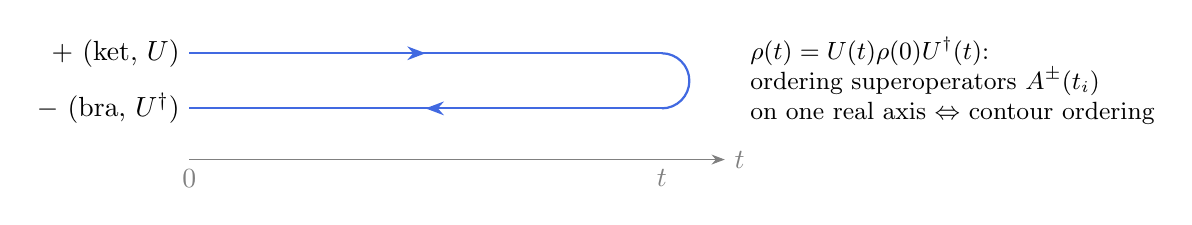
\begin{tikzpicture}[>=Stealth,scale=1.0]
  % contour
  \draw[thick,RoyalBlue,postaction={decorate},decoration={markings,mark=at position 0.5 with {\arrow{>}}}]
      (0,0.35) -- (6,0.35);
  \draw[thick,RoyalBlue] (6,0.35) arc (90:-90:0.35);
  \draw[thick,RoyalBlue,postaction={decorate},decoration={markings,mark=at position 0.5 with {\arrow{>}}}]
      (6,-0.35) -- (0,-0.35);
  \node[left] at (0,0.35) {$+$ (ket, $U$)};
  \node[left] at (0,-0.35) {$-$ (bra, $U^\dagger$)};
  \draw[->,gray] (0,-1.0) -- (6.8,-1.0) node[right] {$t$};
  \node[below,gray] at (0,-1.0) {$0$};
  \node[below,gray] at (6,-1.0) {$t$};
  \node[right,align=left,font=\small] at (7.0,0.0) {$\rho(t)=U(t)\rho(0)U^\dagger(t)$:\\
  ordering superoperators $A^\pm(t_i)$\\ on one real axis $\Leftrightarrow$ contour ordering};
\end{tikzpicture}

\vspace{6pt}
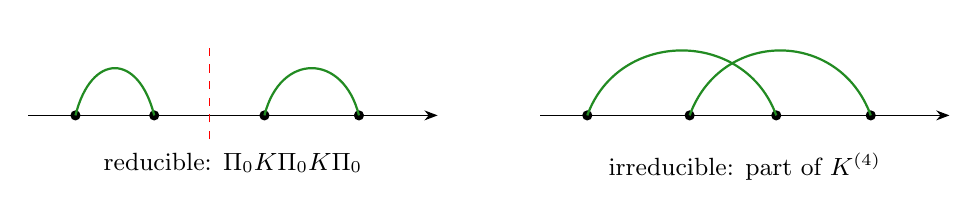
\begin{tikzpicture}[>=Stealth,scale=1.0]
  \tikzset{v/.style={circle,fill=black,inner sep=1.3pt}}
  % reducible
  \draw[->] (0,0)--(5.2,0);
  \foreach \x in {0.6,1.6,3.0,4.2} \node[v] at (\x,0) {};
  \draw[thick,ForestGreen] (0.6,0) .. controls (0.8,0.8) and (1.4,0.8) .. (1.6,0);
  \draw[thick,ForestGreen] (3.0,0) .. controls (3.2,0.8) and (4.0,0.8) .. (4.2,0);
  \draw[dashed,red] (2.3,-0.3)--(2.3,0.9);
  \node[below,font=\small] at (2.6,-0.35) {reducible: $\Pi_0K\Pi_0K\Pi_0$};
  % irreducible
  \begin{scope}[xshift=6.5cm]
  \draw[->] (0,0)--(5.2,0);
  \foreach \x in {0.6,1.9,3.0,4.2} \node[v] at (\x,0) {};
  \draw[thick,ForestGreen] (0.6,0) .. controls (1.0,1.1) and (2.6,1.1) .. (3.0,0);
  \draw[thick,ForestGreen] (1.9,0) .. controls (2.3,1.1) and (3.8,1.1) .. (4.2,0);
  \node[below,font=\small] at (2.6,-0.35) {irreducible: part of $K^{(4)}$};
  \end{scope}
\end{tikzpicture}
\caption{Top: the Keldysh contour. The forward and backward branches are the ket and
bra sides of $\rho$. Bottom: real-time diagrams for the reduced propagator. Vertices are
system superoperators $S^{\cl/\qu}$ and lines are bath contractions ($S$ or $\chi$). A
diagram that can be cut between vertices without cutting a line (red) is reducible. The
NZ kernel collects exactly the irreducible diagrams.}
\label{fig:contour}
\end{figure}

In the interaction picture, $\tilde\rho(t)=T\exp\!\big[\int_0^t\dd s\,\tilde\Lc_I(s)\big]\rho(0)$.
Expanding the time-ordered exponential produces strings of superoperators
$H_I^{\pm}(t_n)\cdots H_I^{\pm}(t_1)$ with $t_n>\dots>t_1$. A ``$+$'' factor sits to the left of
$\rho(0)$ in time order, and a ``$-$'' factor sits to the right in \emph{anti}-time order. This is
precisely the Keldysh contour of \cref{fig:contour}~\cite{Keldysh1964,Schwinger1961}.
Keldysh ordering is therefore nothing more than ordinary time ordering in Liouville space.

\paragraph{Wick's theorem for superoperators.}
For a Gaussian bath, $\Tr_B[\tilde B^{a_n}(t_n)\cdots\tilde B^{a_1}(t_1)\rhoB]$ (with $a_i\in\{\cl,\qu\}$)
factorizes into pairwise contractions. For $t>s$ these are
\begin{equation}
  \Tr_B[B^{\cl}(t)B^{\cl}(s)\rhoB]=S(t-s),\qquad
  \Tr_B[B^{\cl}(t)B^{\qu}(s)\rhoB]=-i\chi(t-s),\qquad
  \Tr_B[B^{\qu}(t)\,\cdot\,]=0.
  \label{eq:contractions}
\end{equation}
This is the familiar Keldysh causality structure: $\avg{\phi_\cl\phi_\cl}\propto D^K$,
$\avg{\phi_\cl\phi_\qu}\propto D^R$, $\avg{\phi_\qu\phi_\qu}=0$~\cite{Kamenev2011}.
By \cref{eq:LIcq}, a $B^\cl$ vertex carries $S^\qu$ and a $B^\qu$ vertex carries $S^\cl$. Hence
\begin{keybox}[System-side Feynman rules]
Noise lines $S(t-s)$ connect $S^\qu(t)$ to $S^\qu(s)$. Response lines $-i\chi(t-s)$ connect
the \emph{later} $S^\qu(t)$ to the \emph{earlier} $S^\cl(s)$. There are no lines of
$\cl$--$\cl$ type on the system side, the analogue of the vanishing $\qu\qu$ Keldysh
propagator. The latest vertex is always a commutator $S^\qu$, which preserves
$\Tr_S$ (trace preservation of $\Pi$).
\end{keybox}
Summed over all pairings, the same rules generate the Feynman--Vernon influence
functional~\cite{FeynmanVernon1963,Grabert1988,Weiss2012}. In Keldysh-rotated variables,
\begin{equation}
  \Phi[s^\cl,s^\qu]=-\int_0^t\!\dd t_1\!\int_0^{t_1}\!\dd t_2\,
  \Big[s^\qu(t_1)S(t_1-t_2)s^\qu(t_2)-i\,s^\qu(t_1)\chi(t_1-t_2)s^\cl(t_2)\Big],
  \label{eq:FV}
\end{equation}
where $s^{\pm}$ are the path variables on the two branches. $S$ is the Feynman--Vernon
noise kernel and $\chi$ the dissipation kernel. For a single Gaussian bath this equation
contains \emph{all} the information that any of the methods below will use.

%=====================================================================
\section{Nakajima--Zwanzig and TCL as Dyson equations}
\label{sec:nz}

\subsection{The NZ equation}
Take $\Pc X=\rhoB\otimes\Tr_B X$ and $\Qc=1-\Pc$~\cite{Nakajima1958,Zwanzig1960,BreuerPetruccione}.
Our assumptions give $\Pc\Lc_I\Pc=0$ and $[\Pc,\Lc_S+\Lc_B]=0$. For a factorized initial
state the inhomogeneous term vanishes, and
\begin{equation}
  \dot\rho_S(t)=\Lc_S\rho_S(t)+\int_0^t\!\dd s\,K(t-s)\,\rho_S(s),\qquad
  K(\tau)X=\Tr_B\!\big[\Lc_I\,\ee^{\Qc\Lc\tau}\,\Qc\Lc_I\,(X\otimes\rhoB)\big].
  \label{eq:NZ}
\end{equation}
In Laplace space, $\hat f(z)=\int_0^\infty\dd t\,\ee^{-zt}f(t)$ and
\begin{equation}
  \boxed{\;\hat\Pi(z)=\frac{1}{z-\Lc_S-\hat K(z)}
  \quad\Longleftrightarrow\quad
  \hat\Pi=\hat\Pi_0+\hat\Pi_0\,\hat K\,\hat\Pi,\qquad \hat\Pi_0=(z-\Lc_S)^{-1}.\;}
  \label{eq:Dyson}
\end{equation}

\subsection{Why \texorpdfstring{$K$}{K} is the irreducible self-energy}
Insert the Wick expansion of \cref{sec:keldysh-rho} into $\Pi(t)$. Every contribution is a
time-ordered string of system superoperators, dressed by contraction lines and
interleaved with $\ee^{\Lc_S\Delta t}$. Now cut the time axis between any two
consecutive vertices. If no line crosses the cut, the bath returns to $\rhoB$ there
and the diagram factorizes as $\cdots\Pi_0\,\Pc\cdots$. The factor $\Qc$ inside
$\ee^{\Qc\Lc\tau}\Qc$ in \cref{eq:NZ} removes exactly these returns to $\rhoB$. Hence
\begin{keybox}[Identity]
$K=\sum\{\text{irreducible real-time diagrams}\}$, and \cref{eq:Dyson} is the Dyson
equation of Keldysh real-time diagrammatics for the reduced density
matrix~\cite{SchoellerSchon1994,Konig1996,Schoeller2009,LeijnseWegewijs2008,Timm2008}.
\end{keybox}
For fermionic reservoirs the same statement holds, with sign factors from line
crossings; this is the Schoeller--Sch\"on setting. For non-Gaussian baths, higher
cumulants replace pairwise lines. In both cases irreducibility is defined with respect
to the \emph{reference state} $\rhoB$ that appears in $\Pc$. Changing the projector (for
example, to correlated projectors) changes the kernel.

\subsection{Second order: the Keldysh structure made explicit}
At order $\Lc_I^2$ we can drop $\Qc$ in \cref{eq:NZ} because $\Pc\Lc_I\Pc=0$. Using
\cref{eq:LIcq,eq:contractions},
\begin{equation}
  \boxed{\;K^{(2)}(\tau)=-\sum_{\alpha\beta}S^\qu_\alpha\,\ee^{\Lc_S\tau}
  \Big[S_{\alpha\beta}(\tau)\,S^\qu_\beta-i\,\chi_{\alpha\beta}(\tau)\,S^\cl_\beta\Big].\;}
  \label{eq:K2}
\end{equation}
Written out, this is the familiar Born kernel
\begin{equation}
K^{(2)}(\tau)X=-\sum_{\alpha\beta}\big[S_\alpha,\ee^{\Lc_S\tau}\big(C_{\alpha\beta}(\tau)S_\beta X-C_{\beta\alpha}(-\tau)XS_\beta\big)\big].
\end{equation}
The rotated form in \cref{eq:K2} shows the two separate bath inputs, noise and response,
and so connects directly to the influence functional~\eqref{eq:FV}.

\paragraph{Markov and Lindblad limits.}
Replace $\rho_S(s)\to\ee^{-\Lc_S(t-s)}\rho_S(t)$ and extend the upper limit of integration to
$\infty$; this gives Redfield's equation. The secular approximation then gives the
Gorini--Kossakowski--Sudarshan--Lindblad (GKSL) form, with rates set by
$C(\omega)=S(\omega)+\chi''(\omega)$, which equals $2\chi''(\omega)[1+n_B(\omega)]$ in equilibrium. In the field-theory
language, a Lindblad equation corresponds to a Keldysh action with time-local
$\Sigma^R$ and frequency-independent $\Sigma^K$~\cite{Sieberer2016}:
\begin{equation}
  S_K=\int\!\dd t\Big[\bar\psi_+ i\partial_t\psi_+-\bar\psi_- i\partial_t\psi_- -H_++H_-
  -i\sum_j\Big(L_{j+}\bar L_{j-}-\tfrac12\big(\bar L_{j+}L_{j+}+\bar L_{j-}L_{j-}\big)\Big)\Big].
\end{equation}

\subsection{TCL and the NZ--TCL map}
The time-convolutionless (TCL) generator~\cite{Shibata1977,Chaturvedi1979} is
$\Gc(t)=\dot\Pi(t)\Pi(t)^{-1}$, defined wherever $\Pi(t)$ is invertible. Substituting \cref{eq:NZ} gives
\begin{equation}
  \Gc(t)=\Lc_S+\int_0^t\!\dd s\,K(t-s)\,\Pi(s)\,\Pi(t)^{-1},
  \label{eq:TCLNZ}
\end{equation}
an exact relation. Nestmann, Bruch and Wegewijs turn it into a fixed-point equation that
generates $\Gc$ from $K$ (and conversely)~\cite{Nestmann2021}. Reimer
\emph{et al.}\ compare five exact formulations, with attention to complete positivity
and divisibility~\cite{Reimer2019}. Three facts are worth keeping in mind:
\begin{itemize}\itemsep0pt
\item Truncating $K$ and truncating $\Gc$ at the same order are \emph{different} approximations.
  They agree at second order and differ from fourth order on~\cite{LeijnseWegewijs2008,Timm2008,Timm2011}.
\item $\Gc(t)$ can be singular when $\Pi(t)$ is not invertible (for example, the resonant damped
  Jaynes--Cummings model at strong coupling~\cite{BreuerPetruccione}); $K$ never is.
  ``Local versus nonlocal'' is therefore a question about the \emph{representation}, not
  about the physics~\cite{ChruscinskiKossakowski2010}.
\item With correlated initial states, the NZ inhomogeneity reappears. On the Keldysh side
  it corresponds to the imaginary-time (Matsubara) leg of the Kadanoff--Baym
  contour~\cite{StefanucciVanLeeuwen}.
\end{itemize}

%=====================================================================
\section{Mori's projection and the retarded self-energy}
\label{sec:mori}

\subsection{Generalized Langevin equation}
Mori projects \emph{operators}, not states~\cite{Mori1965,ZwanzigBook,Forster1975}. Let
$\dot A=i[H,A]\equiv i\mathsf{L}A$, choose an inner product $(X,Y)$, and set
$\mathsf{P}X=A\,(A,A)^{-1}(A,X)$, $\mathsf{Q}=1-\mathsf{P}$. Then, exactly,
\begin{equation}
  \dot A(t)=i\Omega\,A(t)-\int_0^t\!\dd s\,M(t-s)\,A(s)+F(t),\qquad
  F(t)=\ee^{i\mathsf{QL}t}\,\mathsf{Q}\,i\mathsf{L}A,
  \label{eq:GLE}
\end{equation}
with $i\Omega=(A,i\mathsf{L}A)(A,A)^{-1}$ and memory $M(t)=(F,F(t))(A,A)^{-1}$
(Kubo's second FDT~\cite{Kubo1966}). The random force satisfies $(A,F(t))=0$, so the correlation
$C(t)=(A,A(t))$ obeys
\begin{equation}
  \hat C(z)=\frac{1}{z-i\Omega+\hat M(z)}\,C(0),
  \label{eq:MoriDyson}
\end{equation}
which again has Dyson form.

\subsection{Worked example: the resonant level}
Take $H=\varepsilon c^\dagger c+\sum_k\varepsilon_kd_k^\dagger d_k+\sum_k(V_kc^\dagger d_k+\text{h.c.})$,
$A=c$, and the anticommutator inner product $(X,Y)=\avg{\{X^\dagger,Y\}}$, so that $(c,c)=1$. Then
$C(t)=\avg{\{c^\dagger,c(t)\}}$ and $G^R(t)=-i\theta(t)C(t)$. One finds $i\Omega=-i\varepsilon$ and
$F(0)=-i\sum_kV_kd_k$. The $\mathsf{Q}$-projected dynamics evolves $d_k$ freely, so
$M(t)=\sum_k|V_k|^2\ee^{-i\varepsilon_kt}$. Continuing $z\to-i\omega+0^+$ in \cref{eq:MoriDyson},
\begin{equation}
  G^R(\omega)=\frac{1}{\omega-\varepsilon-\Sigma^R(\omega)},\qquad
  \boxed{\;\Sigma^R(\omega)=-i\,\hat M(-i\omega+0^+)=\sum_k\frac{|V_k|^2}{\omega-\varepsilon_k+i0^+}.\;}
\end{equation}
This is the exact hybridization self-energy. For interacting systems the same
construction reproduces the Dyson equation: the static (Hartree--Fock) part of $\Sigma$
sits in $\Omega$ and the dynamical part in $M$~\cite{Fulde1995}. Mori's continued fraction,
obtained by iterating the projection, is the recursion method for $G^R$.

\subsection{What Mori does \texorpdfstring{\emph{not}}{not} give you, and where Keldysh comes in}
\Cref{eq:MoriDyson} determines response functions, that is, the retarded sector. In
equilibrium, the FDT then fixes the Keldysh component,
$G^K=(1-2f)(G^R-G^A)$. Out of equilibrium, occupations, currents and noise live in
$G^{<}$ (equivalently $G^K$), which the retarded function alone does not determine. In
steady state without bound states, $G^<=G^R\Sigma^<G^A$~\cite{JauhoWingreenMeir1994,RammerSmith1986}.
Three routes supply the missing information:
\begin{enumerate}\itemsep0pt
\item \emph{Density-matrix projection} (NZ, \cref{sec:nz}), which evolves the one-time state.
\item \emph{Kadanoff--Baym equations}~\cite{KadanoffBaym,StefanucciVanLeeuwen} for two-time
  $G^{\lessgtr}$, reduced to one-time kinetic equations by the generalized Kadanoff--Baym
  ansatz (GKBA)~\cite{Lipavsky1986}:
  \begin{equation}
    G^{\lessgtr}(t,t')\approx i\big[G^R(t,t')\,G^{\lessgtr}(t',t')-G^{\lessgtr}(t,t)\,G^A(t,t')\big].
  \end{equation}
  GKBA plays the role of the projection onto one-time quantities, here the one-body
  density matrix $\rho^{(1)}(t)=-iG^<(t,t)$.
\item \emph{Time-dependent Mori projections} with nonstationary reference
  states~\cite{Grabert1982}. These produce two-time memory kernels and are closer in
  spirit to Kadanoff--Baym.
\end{enumerate}

\subsection{Generalized Langevin equation \texorpdfstring{$\leftrightarrow$}{<->} Keldysh saddle point}
For a linear bath coupled to a coordinate $x$ (Caldeira--Leggett /
Ford--Kac--Mazur~\cite{CaldeiraLeggett1983,FordKacMazur1965}), apply a
Hubbard--Stratonovich decoupling to the $\qu\qu$ noise term in \cref{eq:FV} with a real
field $\xi$. The equation of motion $\delta/\delta x^\qu=0$ is then the quantum Langevin
equation
\begin{equation}
  m\ddot x^\cl+V'(x^\cl)-\int_{-\infty}^{t}\!\dd s\,\chi(t-s)\,x^\cl(s)=\xi(t),\qquad
  \avg{\xi(t)\xi(s)}=S(t-s),
\end{equation}
which is Mori's \cref{eq:GLE} for $A=x$, with $M\leftrightarrow\chi$ and $F\leftrightarrow\xi$.
Kubo's second FDT and the equilibrium relation between $\Sigma^K$ and $\Sigma^R$ are the same
statement~\cite{Kamenev2011,Weiss2012}.

%=====================================================================
\section{Dictionary}
\label{sec:dictionary}

\begin{center}
\small
\renewcommand{\arraystretch}{1.25}
\begin{tabularx}{\textwidth}{>{\raggedright\arraybackslash}X>{\raggedright\arraybackslash}X>{\raggedright\arraybackslash}X}
\toprule
\textbf{Keldysh / NEGF} & \textbf{Nakajima--Zwanzig / TCL} & \textbf{Mori} \\
\midrule
Contour branches $\pm$; $\cl/\qu$ rotation & Left/right superoperators; $A^\cl=\frac12\{A,\cdot\}$, $A^\qu=[A,\cdot]$ & --- \\
$D^R$ (bath response) & $\chi$ on $\qu$--$\cl$ lines & damping kernel in $M$ \\
$D^K$ (bath noise) & $S$ on $\qu$--$\qu$ lines & random-force statistics $(F,F(t))$ \\
Dyson: $G=G_0+G_0\Sigma G$ & $\hat\Pi=\hat\Pi_0+\hat\Pi_0\hat K\hat\Pi$ & $\hat C=[z-i\Omega+\hat M]^{-1}C(0)$ \\
Irreducible self-energy & NZ kernel $K$ (irreducible diagrams) & memory function $M$ ($\propto\Sigma^R$ for $A=c$) \\
Single-particle space & Liouville space of $\rho_S$ (dimension $d^2$) & span of chosen operators \\
Retarded \emph{and} Keldysh sectors & full one-time state & retarded sector only (out of eq.) \\
Kadanoff--Baym $\to$ GKBA & NZ $\to$ TCL (one-time closure) & time-dependent projections \\
Matsubara leg (initial correlations) & inhomogeneous term & initial-value dependence of $F$ \\
Saddle point + Hubbard--Stratonovich $\Rightarrow$ Langevin & --- & GLE \eqref{eq:GLE} \\
Local $\Sigma^R$, constant $\Sigma^K$ & GKSL / Lindblad & Markovian $M(t)\propto\delta(t)$ \\
\bottomrule
\end{tabularx}
\end{center}
Each approach has its natural territory. Keldysh field theory suits many-body problems,
renormalization group, large-$N$ and loop expansions, and self-consistent schemes
(e.g.\ open-system DMFT~\cite{Scarlatella2021}). NZ/TCL suits small systems, where
questions about complete positivity, divisibility and memory are posed directly on $\Pi$.
Mori suits the choice of relevant slow variables and continued-fraction approximations.
Exact numerical bridges exist: memory kernels can be extracted from projection-free
inputs~\cite{ShiGeva2003} or from exact impurity solvers~\cite{CohenRabani2011,Kidon2015}, and
hierarchical equations of motion (HEOM)~\cite{Tanimura2020} and process
tensors~\cite{Pollock2018} give independent exact references.

%=====================================================================
\section{A sensing-flavoured example: pure dephasing done three ways}
\label{sec:sensing}

Take a qubit sensor $H_S=\frac{\omega_0}{2}\sigma_z$ with $H_I=\frac12\sigma_z\otimes B$, a Gaussian bath,
and a factorized initial state. On the coherence $X=\ket0\bra1$,
$S^\qu X=X$ and $S^\cl X=0$ (for $S=\sigma_z/2$). By \cref{eq:K2}, every response line then
vanishes and only noise lines survive. Summing all pairings gives the exact result
\begin{equation}
  \rho_{01}(t)=\rho_{01}(0)\,\ee^{-i\omega_0t}\,\ee^{-\Gamma(t)},\qquad
  \Gamma(t)=\int_{-\infty}^{\infty}\!\frac{\dd\omega}{2\pi}\,\frac{S(\omega)}{\omega^2}\,F(\omega,t),
  \label{eq:filter}
\end{equation}
with $F=1-\cos\omega t$ for free induction decay. For a pulse sequence with sign function
$y(s)=\pm1$, $F(\omega,t)=\frac{\omega^2}{2}\big|\int_0^t y(s)\ee^{i\omega s}\dd s\big|^2$, the filter function of
dynamical decoupling and noise spectroscopy~\cite{Cywinski2008,Degen2017}. (Normalizations
differ between papers.) The three descriptions compare as follows:
\begin{itemize}\itemsep0pt
\item \textbf{Keldysh}: \cref{eq:filter} is $\exp$ of the $\qu\qu$ part of the influence
  functional~\eqref{eq:FV}. Only $D^K$ enters, so for pure dephasing a sensor measures the
  symmetrized noise and is blind to $\chi$.
\item \textbf{TCL}: $\Gc_{01}(t)=-i\omega_0-\dot\Gamma(t)$ with $\dot\Gamma(t)=\int_0^t S(\tau)\dd\tau$. TCL2 is
  \emph{exact} here.
\item \textbf{NZ}: $\hat K_{01}(z)=z-1/\hat{\tilde\rho}_{01}(z)$ in the rotating frame is an \emph{infinite}
  series in the coupling. This is the cleanest demonstration that ``order $n$'' means
  different things in different representations.
\end{itemize}
For metrology this matters directly: the time dependence of $\Gamma(t)$ at short times
($\propto t^2$ versus $\propto t$) changes the achievable precision scaling under
non-Markovian noise~\cite{Chin2012}.

%=====================================================================
\section{Self-study plan (about 8 weeks, 6--8 h/week)}
\label{sec:plan}

Each stage has a reading core and a derivation to do on paper. The stages are ordered
so that every bridge is crossed only after both of its ends are familiar.

\begin{center}
\small
\renewcommand{\arraystretch}{1.3}
\begin{tabularx}{\textwidth}{@{}p{1.3cm}>{\raggedright\arraybackslash}p{4.6cm}>{\raggedright\arraybackslash}X@{}}
\toprule
\textbf{Week} & \textbf{Read} & \textbf{Goal / do} \\
\midrule
1 & Breuer--Petruccione Ch.~9~\cite{BreuerPetruccione}; de Vega--Alonso (NZ/TCL
    sections)~\cite{deVega2017}; Nakajima, Zwanzig originals~\cite{Nakajima1958,Zwanzig1960}
  & Derive \cref{eq:NZ,eq:Dyson}. \textbf{Ex.~\ref{ex:K2}.} \\
2 & Zwanzig Ch.~8~\cite{ZwanzigBook}; Mori~\cite{Mori1965}; Kubo~\cite{Kubo1966};
    Forster (memory functions)~\cite{Forster1975}
  & Derive the GLE~\eqref{eq:GLE}; second FDT. \textbf{Ex.~\ref{ex:mori}.} \\
3--4 & Kamenev (contour, Keldysh rotation, dissipative oscillator)~\cite{Kamenev2011};
    Kamenev--Levchenko~\cite{KamenevLevchenko2009}; Rammer--Smith~\cite{RammerSmith1986};
    Stefanucci--van Leeuwen (contour, Langreth rules)~\cite{StefanucciVanLeeuwen}
  & Keldysh rotation; causality structure; Langreth rules; $G^<=G^R\Sigma^<G^A$. \textbf{Ex.~\ref{ex:GLE}.} \\
5 & Feynman--Vernon~\cite{FeynmanVernon1963}; Grabert--Schramm--Ingold~\cite{Grabert1988};
    Weiss~\cite{Weiss2012}; Sieberer--Buchhold--Diehl (Lindblad $\leftrightarrow$ Keldysh)~\cite{Sieberer2016}
  & Derive \cref{eq:FV} and the Keldysh action of a Lindblad equation. \textbf{Ex.~\ref{ex:lindblad}.} \\
6 & Schoeller--Sch\"on~\cite{SchoellerSchon1994}; K\"onig \emph{et al.}~\cite{Konig1996};
    Schoeller review~\cite{Schoeller2009}; Leijnse--Wegewijs~\cite{LeijnseWegewijs2008}; Timm~\cite{Timm2008}
  & The central bridge: prove $K=\sum$(irreducible diagrams). \textbf{Ex.~\ref{ex:irred}.} \\
7 & Timm (TCL to all orders)~\cite{Timm2011}; Reimer \emph{et al.}~\cite{Reimer2019};
    Nestmann--Bruch--Wegewijs~\cite{Nestmann2021}; Lipavsk\'y \emph{et al.}\ (GKBA)~\cite{Lipavsky1986};
    Shi--Geva~\cite{ShiGeva2003}; Cohen--Rabani~\cite{CohenRabani2011}
  & NZ $\leftrightarrow$ TCL map~\eqref{eq:TCLNZ}; GKBA as one-time closure. \textbf{Ex.~\ref{ex:tcl}.} \\
8 & Degen--Reinhard--Cappellaro~\cite{Degen2017}; Cywi\'nski \emph{et al.}~\cite{Cywinski2008};
    Chin--Huelga--Plenio~\cite{Chin2012}
  & Capstone (\cref{ex:capstone}); write up a one-page summary of your own. \\
\bottomrule
\end{tabularx}
\end{center}

\paragraph{Optional extensions.} Gurvitz--Prager infinite-bias Markovianity~\cite{GurvitzPrager1996};
Kidon--Wilner--Rabani exact TCL generator~\cite{Kidon2015}; HEOM~\cite{Tanimura2020};
process tensors~\cite{Pollock2018}; open-system DMFT~\cite{Scarlatella2021}; Grabert's
time-dependent projections~\cite{Grabert1982}.

\subsection*{Exercises}

\begin{exercise}\label{ex:K2}
Starting from \cref{eq:NZ,eq:LIcq}, derive \cref{eq:K2}. Show that $\Tr_S K^{(2)}(\tau)X=0$ for all $X$
and explain this as ``the last vertex is always $S^\qu$''.
\end{exercise}

\begin{exercise}\label{ex:mori}
Reproduce $\Sigma^R=-i\hat M(-i\omega+0^+)$ for the resonant level. Then add an on-site
Hubbard $U$ for a spinful level and identify the Hartree term in $\Omega$.
\end{exercise}

\begin{exercise}\label{ex:GLE}
For Caldeira--Leggett, derive the quantum Langevin equation both from Mori's projection
onto $(x,p)$ and from the Keldysh saddle point with Hubbard--Stratonovich noise. Match
$M\leftrightarrow\chi$ and $(F,F(t))\leftrightarrow S$.
\end{exercise}

\begin{exercise}\label{ex:lindblad}
From the GKSL equation, write the Keldysh action and read off $\Sigma^R$ and $\Sigma^K$ for a
damped cavity mode. Check that they follow from \cref{eq:K2} in the Born--Markov--secular
limit.
\end{exercise}

\begin{exercise}\label{ex:irred}
Prove that $\Pc\Lc_I(\Qc\,\ee^{\Qc\Lc\tau}\Qc)\Lc_I\Pc$ generates exactly the irreducible real-time
diagrams. (Hint: expand $\ee^{\Qc\Lc\tau}$ in $\Lc_I$ and show that every insertion of $\Pc$
corresponds to a cut with no crossing line.) Verify at fourth order by drawing all
diagrams.
\end{exercise}

\begin{exercise}\label{ex:tcl}
For the pure-dephasing model of \cref{sec:sensing}, compute $\hat K_{01}(z)$ to fourth order and
check \cref{eq:TCLNZ}. Then do the damped Jaynes--Cummings model and locate the
singularity of $\Gc(t)$.
\end{exercise}

\begin{exercise}[Capstone]\label{ex:capstone}
Resonant level between two wide-band leads ($\Gamma_L,\Gamma_R$), prepared empty at $t=0$.
(a) Keldysh: compute $n(t)=-iG^<(t,t)$ exactly. (b) NZ: extract the exact memory kernel for
$n(t)$ and show that it becomes time-local in the infinite-bias limit~\cite{GurvitzPrager1996}.
(c) TCL: build $\Gc(t)$ from \cref{eq:TCLNZ} and compare with its perturbative truncations.
(d) Sensing: replace the leads by a Gaussian spin bath coupled via $\sigma_z$ and relate your
kernel to the filter-function formula~\eqref{eq:filter} under a Hahn echo.
\end{exercise}

%=====================================================================
\bibliographystyle{unsrtnat}
\bibliography{refs}

\end{document}
